%! Author = wolfram_e_laube
%! Date = 06.05.24

\item[(c)]
\section*{Exercise 1 Task (c): Sampling and Frequency Analysis}

\subsection*{Objective}
To visually demonstrate the effect of a high sampling rate on a discrete-time signal and confirm the frequency spectrum through FFT analysis.

\subsection*{Theoretical Background}
Sampling a continuous-time signal at a discrete rate preserves the signal's characteristics if the sampling frequency exceeds twice the highest frequency component of the signal.
This practice helps prevent aliasing, ensuring that the discrete representation closely matches the original signal.
FFT analysis of the sampled signal provides a quantitative view of the frequency components, further validating the sampling process.

\subsection*{Signal Sampling and Visualization}
The signal $x(t) = \sin(2\pi 4000t) + \sin(2\pi 6000t)$ is sampled at a rate of 100 kHz.
Figure~\ref{fig:ex1c_signal_sampling} visualizes the continuous and sampled versions to illustrate how the sampled signal closely follows the continuous signal due to adequate sampling rate.

\begin{figure}[h]
    \centering
    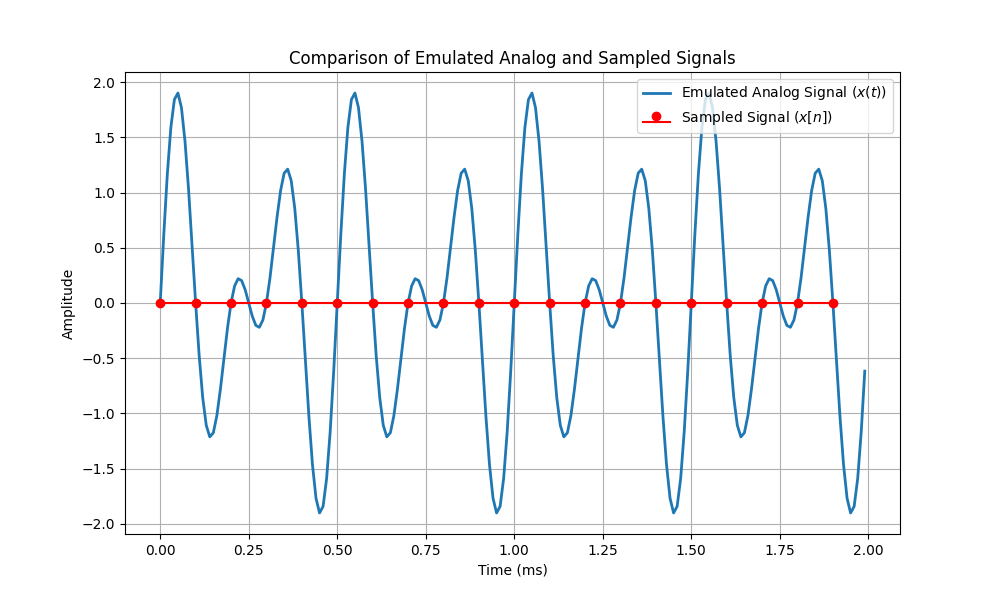
\includegraphics[width=0.8\textwidth]{fig/ex1_c_plot}
    \caption{Overlay of $x(t)$ and $x[n]$}
    \label{fig:ex1c_signal_sampling}
\end{figure}

\subsection*{FFT Analysis}
Following the signal visualization, an FFT is performed on $x[n]$ to analyze its frequency spectrum.
This spectral analysis visualized in Figure~\ref{fig:ex1c_fft_analysis} confirms that the primary frequency components of the signal are captured without distortion.

\begin{figure}[h]
    \centering
    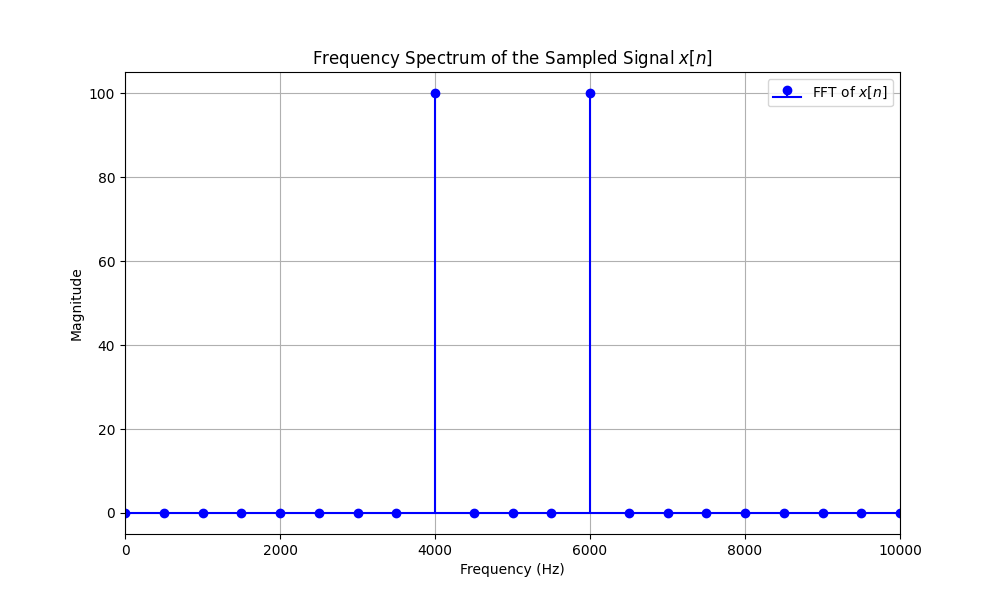
\includegraphics[width=0.8\textwidth]{fig/ex1_c_fft_plot}
    \caption{FFT of $x[n]$}
    \label{fig:ex1c_fft_analysis}
\end{figure}

\subsection*{Conclusion}
Both the time-domain visualization and the frequency-domain analysis confirm that the sampling rate of 100 kHz is sufficient to capture all significant frequency components of $x(t)$. This ensures that the sampled signal $x[n]$ maintains the integrity of the original signal, validating the spectral analysis from Task (b) and demonstrating the effectiveness of proper sampling techniques.
